\chapter{Evaluation}
Um die Rekonstruktionsqualit\"at der Ergebnisse auswerten zu k\"onnen folgt der Vergleich einer normalen MVE Rekonstruktion zu jener verbesserten Variante des Frankfurter AfE-Turms. Zur Evaluation der Resultate dieser Arbeit werden zwei unterschiedliche Datens\"atze verwendet um die Robustheit der algorithmischen Optimierungen zu zeigen, wobei eines den genannten Turm und das andere den Triumphbogen (Arc de Triumphe) in Paris zeigt. Dazu wird zuerst \\
Die Umsetzung des L\"osungsansatzes wurde mittels C++ gel\"ost und aufbauend auf dem MVE Framework und der Qt Bibliothek wurden diese implementiert.

\section{Genauigkeit der Regionsabgrenzung}
Damit auf die Zugeh\"origkeit der einzelnen Bildpunkte zu ihren jeweiligen Geb\"audefassaden geschlossen werden kann, m\"ussen sich diese innerhalb einer der festgelegten Bereiche befinden. Dabei ist ein Simplex die kleinstm\"ogliche Form einer Region, d.h. ein n-dimensionales Polytop\footnote{Polytop beschreibt ein Polygon beliebiger Dimension} mit n+1 Eckpunkten. In dem Fall m\"ussen mindestens drei Eckpunkte pro Region gegeben sein um in der zweidimensionalen Ebene eine Fl\"ache zu definieren. Dahingegen ist die Anzahl der Eckpunkte nach oben hin unbeschr\"ankt. \\
Das Regionierungsverfahren ist in der Lage sowohl konvexe als auch konkave Polygone zu behandeln. Sind Regionen an ihren Kanten zu umgebenden Bildbereichen visuell unterscheidbar und dessen Bildelemente zugeh\"orig identifizierbar, gen\"ugt zur Umrandung einer Region auch lediglich eine konvexe H\"ulle aller relevanten Bildpunkte. Die detailgenaue Segmentierung konkaver Polygone ist meist nur innerhalb homogener Bildbereiche n\"otig. 

\begin{figure}[h]
\centering
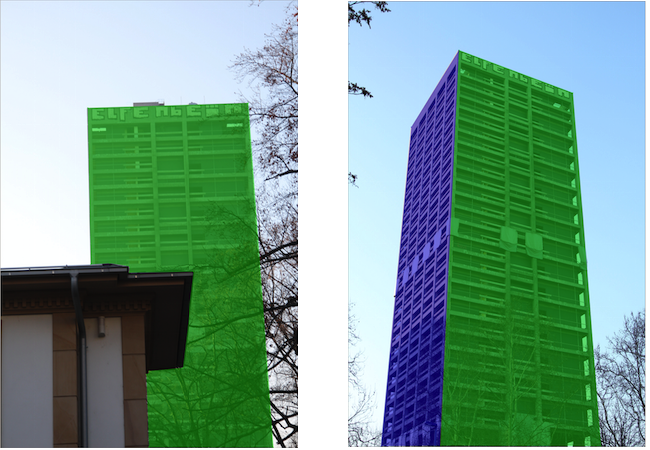
\includegraphics[width=0.9\textwidth]{gfx/konvexkonkav.png}
\caption[Links: Konkave Regionierung Rechts: Konvexe Regionierung]{Links: Konkave Regionierung Rechts: Konvexe Regionierung}
\label{gr:konreg}
\end{figure}
\FloatBarrier

\section{Auswertung regionierter Rekonstruktionen}

In diesem Abschnittl werden die Ergebnisse und Einfl\"usse der Regionierung  auf eine Rekonstruktion zweier Datens\"atze (AfE-Turm in Abschnitt 5.5.1 und der Triumpfbogen, Paris in Abschnitt 5.5.2) vorgestellt und mit den Ergebnissen ohne eine vorherige Regionierung verglichen.

\subsection{AfE-Turm}
Zu Beginn dieses Projektes existierte eine fehlerhafte Rekonstruktion, mit unzureichender Bildqualit\"at. Die Darstellung der unzureichenden Rekonstruktion, die Ausgangspunkt dieses Projektes war, wurde bereits in den vorherigen Kapiteln gezeigt, jedoch in texturierter Form.

\begin{figure}[h]
\centering
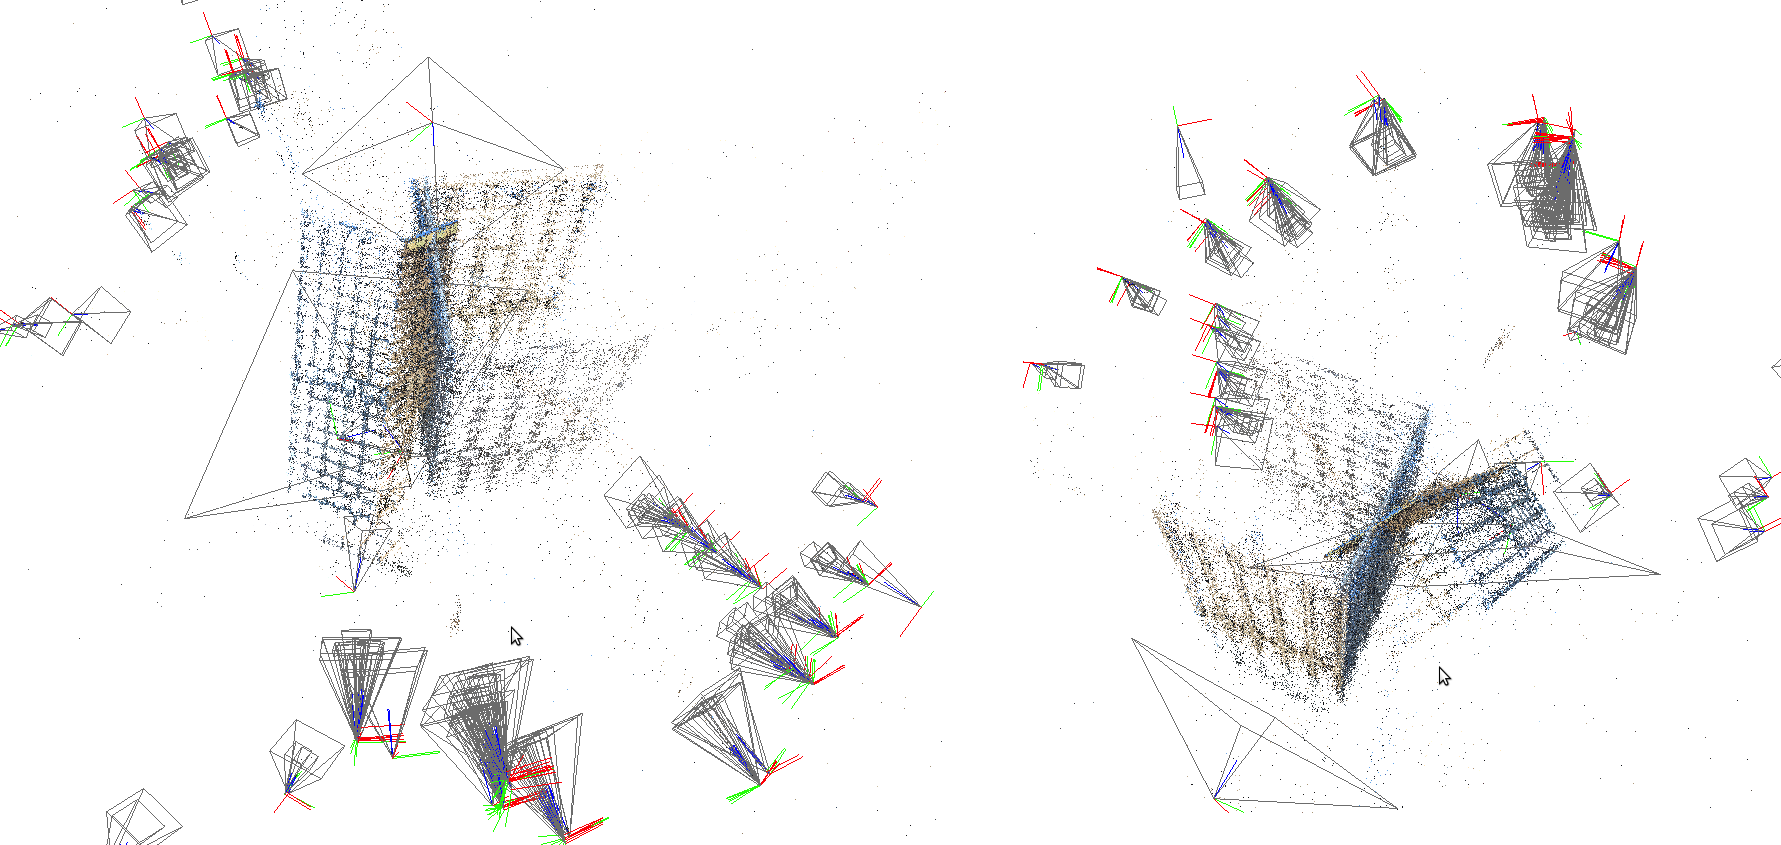
\includegraphics[width=0.9\textwidth]{gfx/Evaluation/prePointcloud_AfEboth.png}
\caption[Punktwolken Drauf- und Seitenansicht der mangelhaften Rekonstruktion]{Punktwolken Drauf- und Seitenansicht der mangelhaften Rekonstruktion}
\label{gr:seitefehler}
\end{figure}
\FloatBarrier

Der anf\"angliche Matchingansatz wurde erweitert, sodass dieser weitere Parameter bez\"uglich der Regionierung ber\"ucksichtigt und das vorher auftretende Artefaktverhalten reduziert. Die Qualit\"at dieses Verfahrens soll hier im Folgenden beurteilt werden. Dazu dienen reale Messdaten des behandelten Frankfurter AfE-Turms, sowie ein Datensatz des Arc de Triomphe in Paris. Als Vergleich der Qualit\"at werden Rekonstruktionen mit und ohne diese erweiterte Methode herangezogen. \\
Stellt man die Ergebnisse eines unbehandelten mit denen eines regionierten Datensatzes gegen\"uber, lassen sich deutliche Unterschiede erkennen. Im ersten Ansatz wird die Rekonstruktion auf geometrische Korrektheit der einzelnen Fassaden \"uberpr\"uft, wobei Positionierung und Orientierung der Geb\"audeseiten f\"ur ein brauchbares Ergebnis stimmen m\"ussen. 

\begin{figure}[h]
\centering
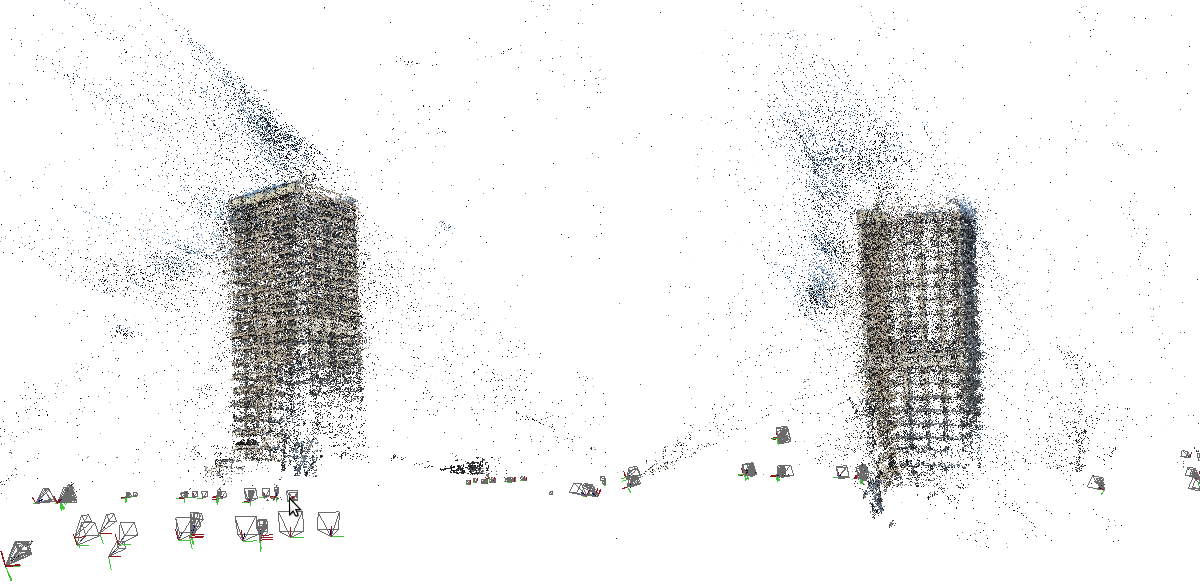
\includegraphics[width=0.9\textwidth]{gfx/Evaluation/finalPointcloud_AfE.png}
\caption[Die Seitenansicht einer Rekonstruktion eines zuvor regionierten Datensatzes]{Die Seitenansicht einer Rekonstruktion eines zuvor regionierten Datensatzes}
\label{gr:seitereg}
\end{figure}
\FloatBarrier

\begin{figure}[h]
\centering
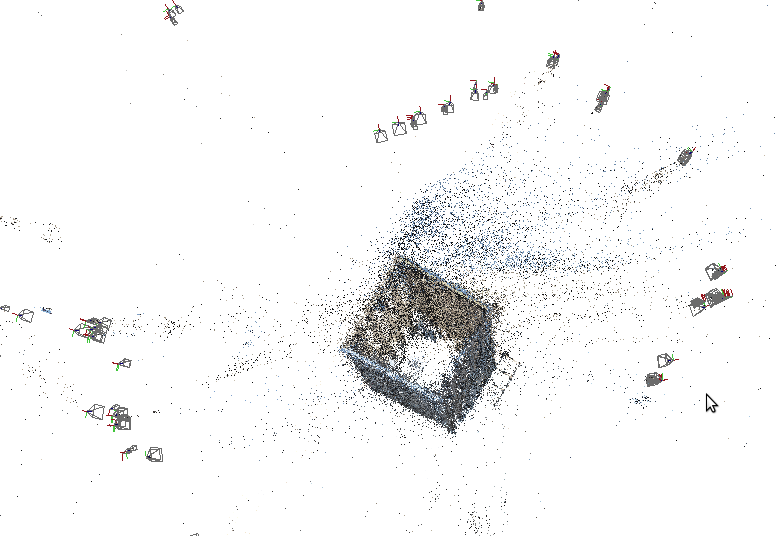
\includegraphics[width=0.9\textwidth]{gfx/Evaluation/finalPointcloud_Top_AfE.png}
\caption[Die Draufsicht einer Rekonstruktion eines zuvor regionierten Datensatzes]{Die Draufsicht einer Rekonstruktion eines zuvor regionierten Datensatzes}
\label{gr:draufreg}
\end{figure}
\FloatBarrier

Neben der nun geometrisch korrekten Ausrichtung der einzelnen Fassaden, bezeugt auch die Anordnung der einzelnen Kameras ein sinnvolles Resultat. Durch das Regioning-Plugin ist UMVE in der Lage vorher falsche Kameraparameter zu korrigieren und die Szene fehlerfrei darzustellen.\\
Insgesamt hat das gezeigte Verfahren Rekonstruktionsfehler entfernt und mehr 3D-Punkte an korrekten Stellen produziert. Hinzu kamen lediglich einige Abbildungen des Himmels, die durch Verdeckungen vereinzelter B\"aume entstanden.

\begin{figure}[h]
\centering
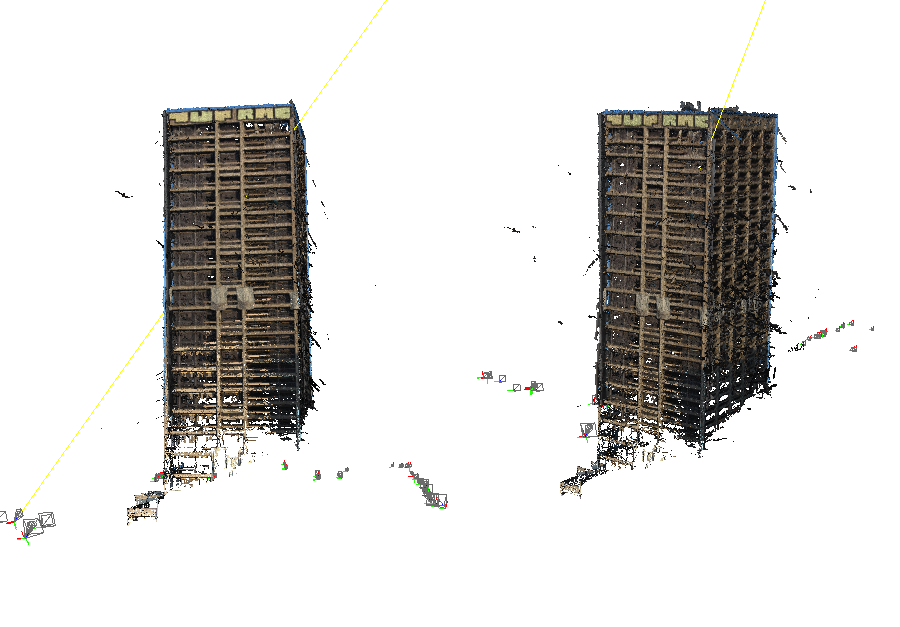
\includegraphics[width=0.9\textwidth]{gfx/Evaluation/finalReconstruction_AfE.png}
\caption[Zwei Seitenansichten einer fehlerfreien Rekonstruktion mit Hilfe des Regioning-Plugins]{Zwei Seitenansichten einer fehlerfreien Rekonstruktion mit Hilfe des Regioning-Plugins}
\label{gr:seitezwei}
\end{figure}
\FloatBarrier

\subsection{Arc de Triomphe}

Als zweiter Datensatz wurde der Arc de Triomphe, Paris gew\"ahlt. Dessen Vorder- und R\"uckseite sind schwierig zu unterscheiden, wodurch sich vermuten l\"asst, dass hier eine Regionierung zu einem besseren Ergebnis f\"uhrt.\\
Tats\"achlich ist es so, dass der Algorithmus bei einer Rekonstruktion ohne Regionierung die Vorder- und R\"uckseite des Triumpfbogens nicht unterscheiden kann und zwischen diesen Matches findet (siehe Abbildung \ref{gr:matchohne}).\\
Durch die Regionierung der Bilddaten und den Ausschluss unzul\"assiger Korrespondenzen ist folglich die Anzahl der detektierten Matches verh\"altnism\"a\ss ig geringer, da fehlerhafte als auch region\"ubergreifende aussortiert wurden. Die folgenden Abbildungen veranschaulichen die Auswirkung regionierter Eingabedaten und unbehandelter in Bezug auf die erfassten Matches.

\begin{figure}[h]
\centering
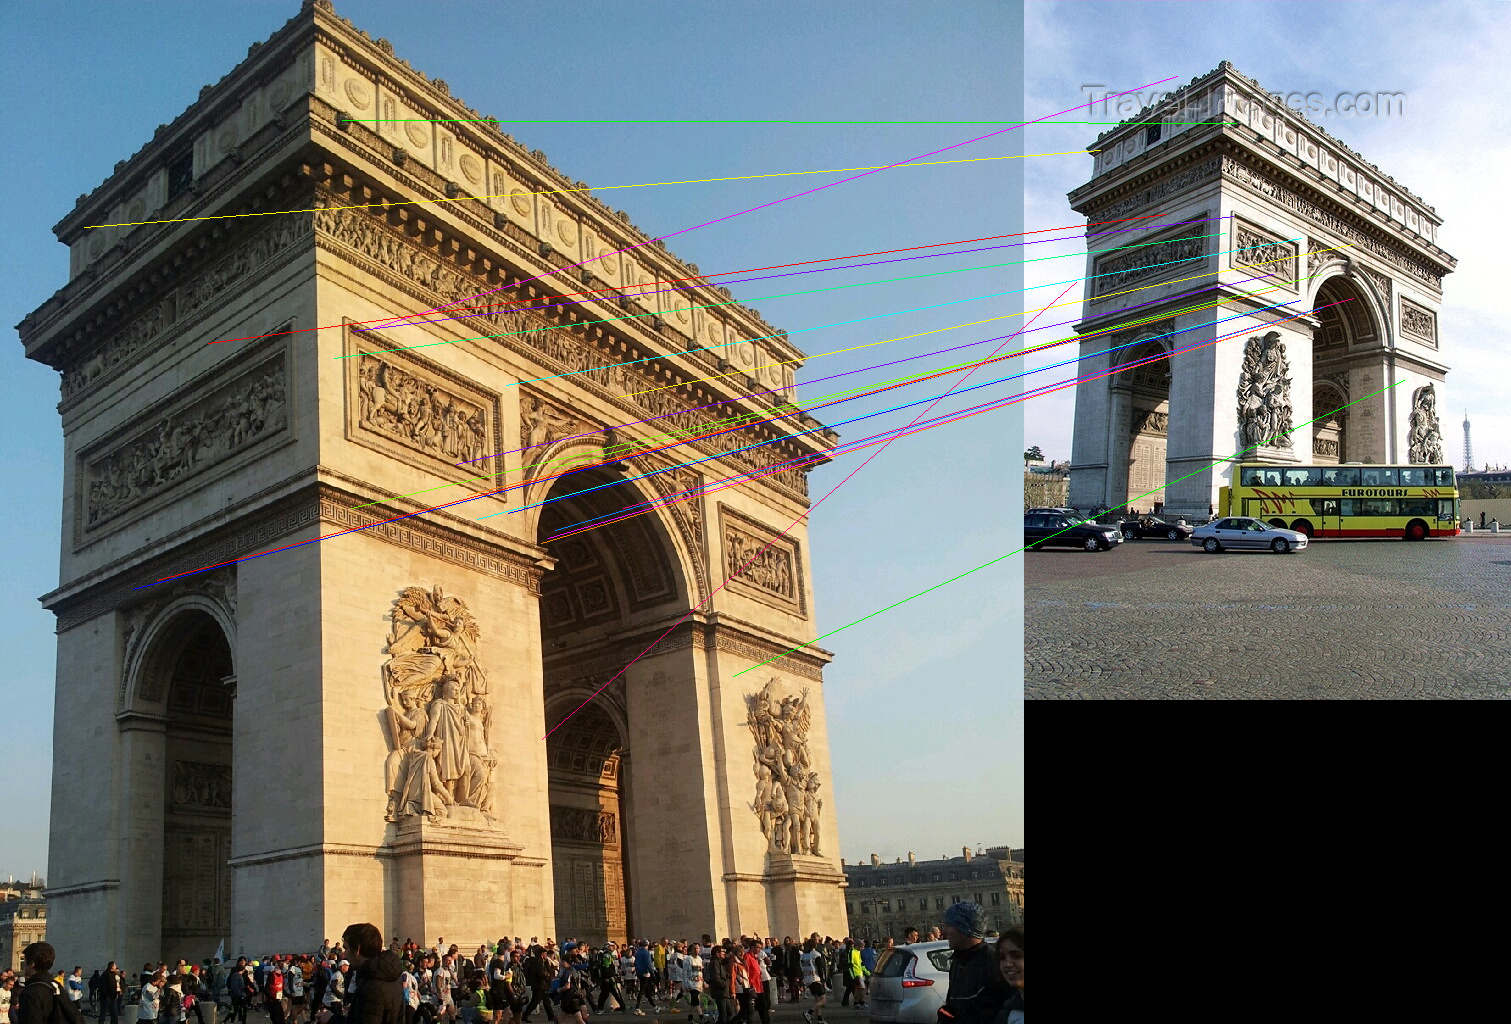
\includegraphics[width=0.9\textwidth]{gfx/Matchingpaare/matching_109_107.png}
\caption[Gefundene Matches zweier unterschiedlicher Seiten ohne Regionierung]{Gefundene Matches zweier unterschiedlicher Seiten ohne Regionierung}
\label{gr:matchohne}
\end{figure}
\FloatBarrier

\begin{figure}[h]
\centering
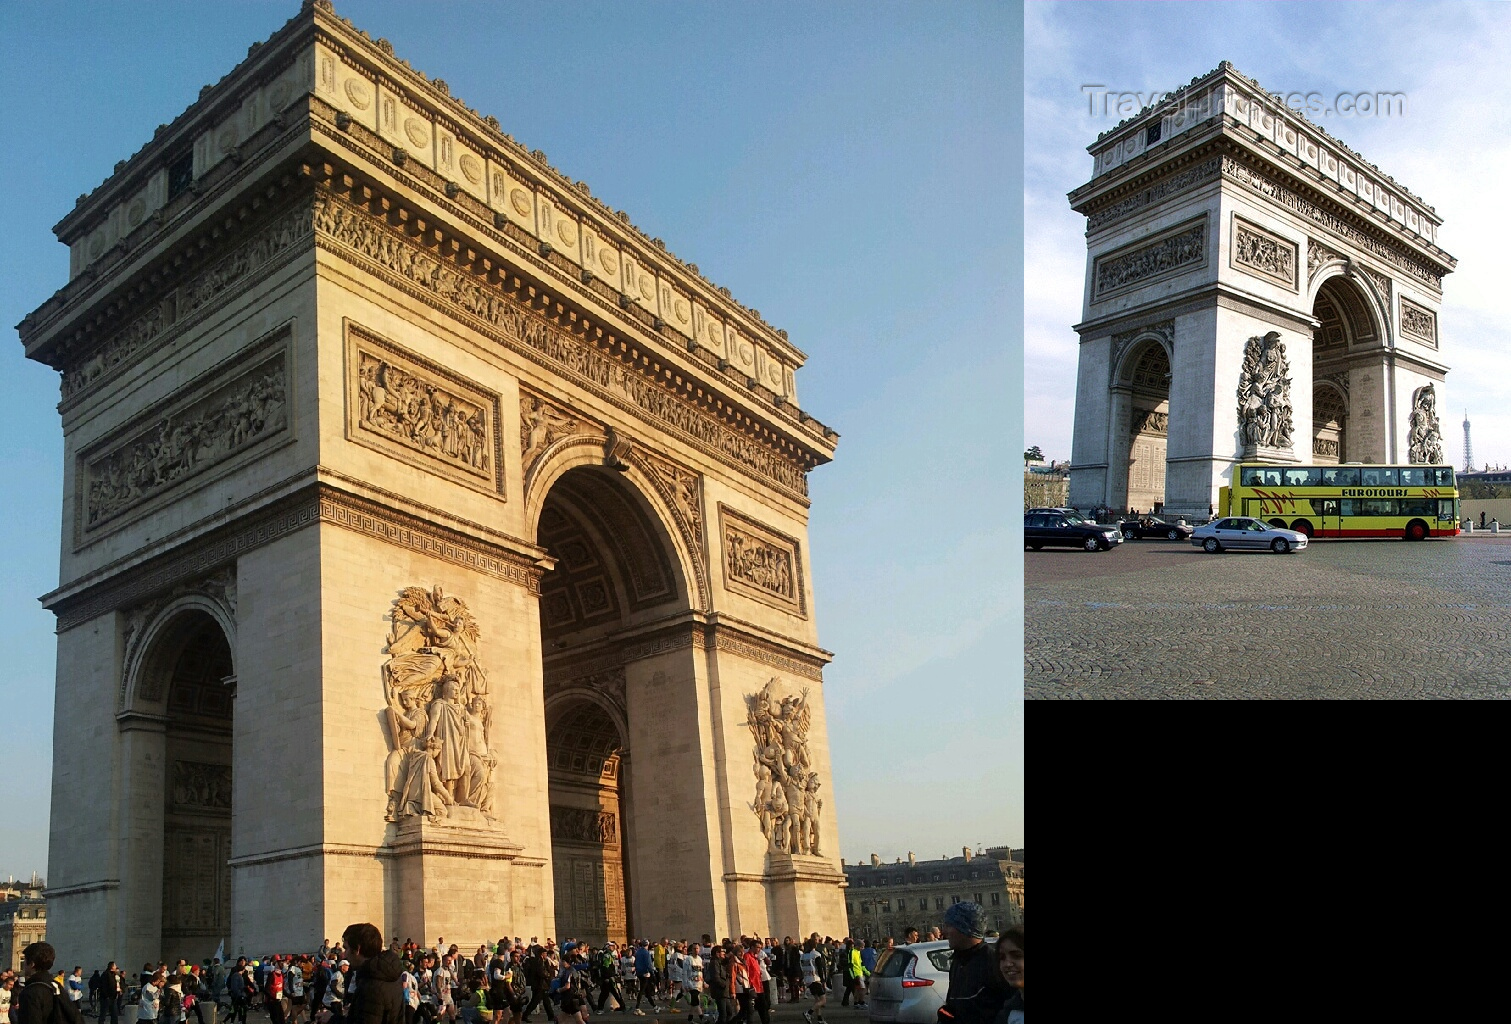
\includegraphics[width=0.9\textwidth]{gfx/Matchingpaare/region_109_107.png}
\caption[Gefundene Matches zweier unterschiedlicher Seiten mit Regionierung]{Gefundene Matches zweier unterschiedlicher Seiten mit Regionierung}
\label{gr:matchmit}
\end{figure}
\FloatBarrier

Dadurch ist eine Unterscheidung zwischen Vorder- und R\"uckseite m\"oglich. Die folgenden Bilder zeigen einen Vergleich zwischen einer Rekonstruktion des Triumpfbogens ohne eine Regionierung (Abbildung \ref{gr:arcohne}und mit einer Regionierung (Abbildung \ref{gr:arcmit}).

\begin{figure}[h]
\centering
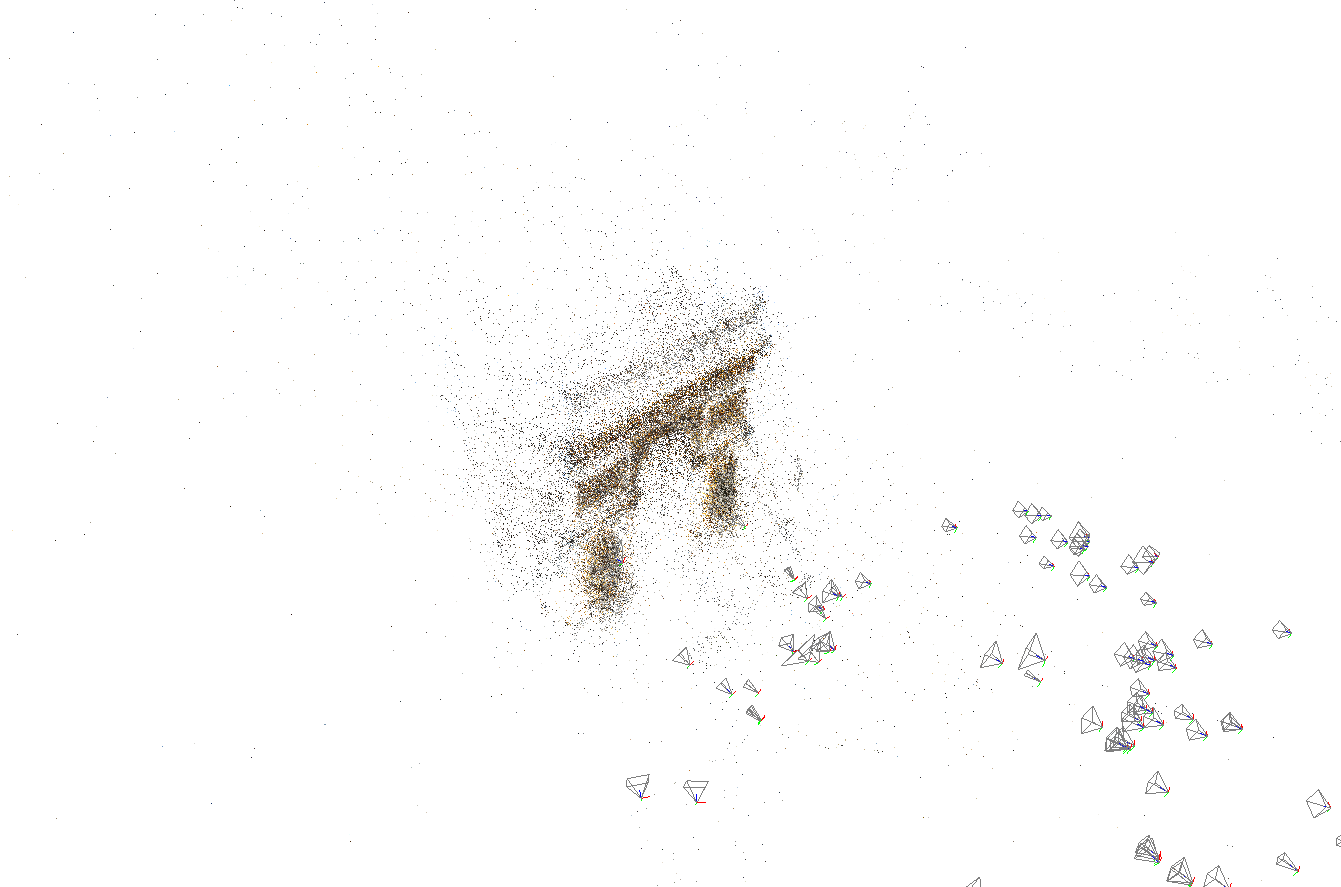
\includegraphics[height=0.34\textheight]{gfx/arcohne.png}
\caption[Rekonstruktion des Triumpfbogens ohne Regionierung]{Rekonstruktion des Triumpfbogens ohne Regionierung}
\label{gr:arcohne}
\end{figure}
\FloatBarrier

\begin{figure}[h]
\centering
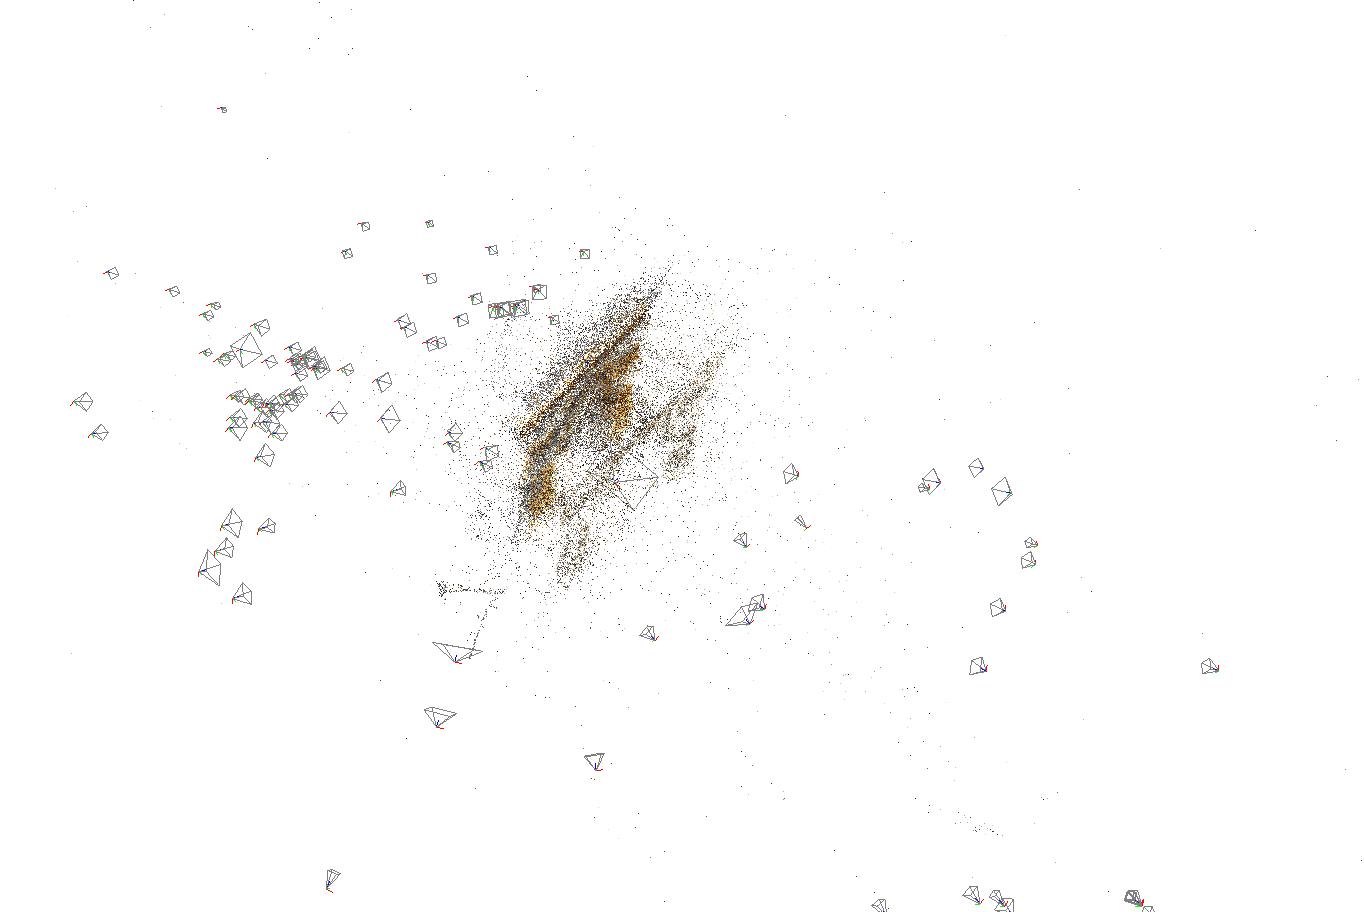
\includegraphics[height=0.34\textheight]{gfx/arcmit.png}
\caption[Rekonstruktion des Triumpfbogens mit Regionierung]{Rekonstruktion des Triumpfbogens mit Regionierung}
\label{gr:arcmit}
\end{figure}
\FloatBarrier

\section{Performanz}
Ohne eine Unterteilung der Eingabebilder in Regionen vergleicht UMVE jedes Feature des ersten Views mit jedem Feature des zweiten Views, was einer quadratischen Laufzeit entspricht. Wurden die Eingabebilder in Regionen unterteilt, werden Features, die in Regionen unterschiedlicher IDs liegen, vom Matchingalgorithmus ausgeschlossen. Da der Matchingalgorithmus bei entsprechend vielen Features eine zeitkritische Komponente der Laufzeit ist, kann so eine Performanzsteigerung durch die Regionierung der Daten resultieren.\\
Die im Folgenden beschriebene Durchf\"uhrung bezieht sich auf den Datensatz des AfE-Turms dessen Eingabebilder jeweils in der Breite und H\"ohe halbiert wurden. Der f\"ur die Ausf\"uhrung verwendete Computer (Intel\textsuperscript{\textregistered} Xeon\textsuperscript{\textregistered} Processor E3-1231 v3
(8M Cache, 3.40 GHz)) erzielte f\"ur eine normale Rekonstruktion mit unbehandeltem Datensatz eine Laufzeit von 50 Minuten. Wohingegen die Durchf\"uhrung mit regionierten Bilddaten eine Dauer von 12 Minuten ergab. Das zeigt eine Verbesserung der Performanz ungef\"ahr um den Faktor 4. F\"ur den Datensatz mit Bildern (verschiedene Aufl\"osungen) des Triumphbogens ergeben sich Laufzeiten von 23 Minuten ohne und 5 Minuten mit Regionierung, was einer Verbesserung der Performanz um den Faktor ca. 4,5 entspricht.